\documentclass{article}


\usepackage{PRIMEarxiv}

\usepackage[utf8]{inputenc} % allow utf-8 input
\usepackage[T1]{fontenc}    % use 8-bit T1 fonts
\usepackage{hyperref}       % hyperlinks
\usepackage{url}            % simple URL typesetting
\usepackage{booktabs}       % professional-quality tables
\usepackage{amsfonts}       % blackboard math symbols
\usepackage{nicefrac}       % compact symbols for 1/2, etc.
\usepackage{microtype}      % microtypography
\usepackage{lipsum}
\usepackage{fancyhdr}       % header
\usepackage{graphicx}       % graphics
\graphicspath{{media/}}     % organize your images and other figures under media/ folder

% paper_setup.tex -- packages and macros used by the text (loaded by one \input line in the preamble).
\usepackage[numbers,sort&compress]{natbib}  % numeric citations; \citet needs unsrtnat
\usepackage{amsmath,amssymb}
\usepackage{array,tabularx}

\newcommand{\mask}{\operatorname{mask}}
\newcommand{\EM}{\mathrm{EM}}
\newcommand{\ED}{\mathrm{ED}}

%Header
\pagestyle{fancy}
\thispagestyle{empty}
\rhead{ \textit{ }} 

% Update your Headers here
\fancyhead[LO]{Running Title for Header}
% \fancyhead[RE]{Firstauthor and Secondauthor} % Firstauthor et al. if more than 2 - must use \documentclass[twoside]{article}



  
%% Title
\title{Substitution Artifacts in Shapley-Based Temporal Attribution:
Characterizing and Correcting Masking-Background Bias on
Mean-Nonstationary Time Series
%%%% Cite as
%%%% Update your official citation here when published 
\thanks{\textit{\underline{Citation}}: 
\textbf{Authors. Title. Pages.... DOI:000000/11111.}} 
}

\author{
  Myroslav Mishchuk \\
  Silesian University of Technology \\ 
  Gliwice, Poland \\
  Lviv Polytechnic National University \\ 
  Lviv, Ukraine \\
  \texttt{myroslav.mishchuk@polsl.pl} \\
   \And
  Rafał Cupek \\
  Silesian University of Technology \\ 
  Gliwice, Poland\\
  \texttt{rafal.cupek@polsl.pl} \\
    \And
  Olena Pavliuk \\
  Silesian University of Technology \\ 
  Gliwice, Poland \\
  Lviv Polytechnic National University \\ 
  Lviv, Ukraine \\
  \texttt{olena.pavliuk@polsl.pl} \\
}


\begin{document}
\maketitle


\begin{abstract}
Shapley-value attribution is the most used way to explain models of industrial data. It removes input elements to measure their importance and replaces them by a background, usually the training mean or zero, since a trained model cannot receive an incomplete input. We show that a single background is the best substitute only for mean-stationary data, whereas models of time series whose mean component follows a system's state read that state; substitutes then lie far from the observations wherever the mean component is far from the background. We characterize six substitution artifacts this can produce, each with an instrument introduced here, and propose trend-aware backgrounds, which condition the substitute on a state estimated from past observations, without a generative model. Since each background has its own correct attribution, recurrent models are trained to reproduce a known function on a testbed calibrated to three battery datasets, which separates the distortion a background causes, a measure introduced here, from the information it removes. Under the training-mean background, \textbf{[RESULT: distortion and its relation to the substitution distance]}, indicating that \textbf{[RESULT: what this means for the stationarity assumption]}. Trend-aware backgrounds \textbf{[RESULT: distortion and explained prediction against unconditional backgrounds and a learned imputer]}, indicating that \textbf{[RESULT: when conditioning on the state suffices]}. On remaining-useful-life models of generated and measured battery data, \textbf{[RESULT: whether the signatures recur]}. In practice, the instruments show whether a background distorts an attribution, and trend-aware backgrounds replace the default background when battery remaining useful life is explained.
\end{abstract}


% keywords can be removed
\keywords{explainable AI \and Shapley values \and temporal attribution \and time series \and mean-nonstationarity \and remaining useful life}


%==============================================================================================
\section{Introduction}
\label{sec:intro}
%==============================================================================================

SHAP \citep{lundberg2017unified} is the explanation method most used in published applications of explainable AI. In a systematic review of 102 studies of explainable predictive maintenance, it was by far the most used method \citep{cummins2024explainable}; across 512 recent applications of explainable AI, it was the most common explanation technique, used in about a third of them \citep{saarela2024recent}; and in explainable forecasting of energy time series, post hoc methods, SHAP in particular, dominate \citep{arabzadeh2025four}. For sequence models, TimeSHAP carries SHAP over to sequences \citep{bento2021timeshap} and assigns to each element of an input window, one channel at one position, a share of the model's output. The share is obtained by removing elements and observing how the output changes. Since a trained model cannot receive an input with elements missing, removal is simulated by substitution: the removed elements take the values of a background, and the model is evaluated on the result. A weakness of this substitution therefore affects the attributions that most practitioners compute.

The background is left to the user. TimeSHAP describes it as an uninformative input, often the zero vector or the average feature values of the dataset \citep{bento2021timeshap}. Later temporal Shapley methods note that the effect of background selection remains understudied \citep{nguyen2025tshap} and find that attributions change when the background changes \citep{kim2026groupsegment, papadeas2026empirical}. Beyond sensitivity, the background also fixes which quantity the attribution explains. Shapley values sum to the difference between the model's output on the input and on the fully substituted input \citep{sundararajan2020many}, so different backgrounds answer different questions about the same prediction \citep{merrick2020explanation, mamalakis2023carefully}. Whether a background serves its question well depends, in turn, on how the model responds to the inputs that substitution creates.

On mean-nonstationary data, whose mean component changes along the sequence, this response becomes systematic. Masking element $(u,c)$ with the background value $b_c$ perturbs the input by the substitution distance $|x_{u,c}-b_c|$. Writing each observation as its mean component plus localized patterns and noise, the systematic part of this distance is the distance between the mean component and the background. An unconditional background stays the same at every state that the sequence passes through, whereas the mean component changes with the state, so the systematic distance is near zero only where the mean component is near the background and grows with their difference. A coalition then combines observed values from one state with substitutes that correspond to another, and the model is evaluated on combinations that its training data do not contain. There, the training data do not constrain the model's output. Shapley values computed from such evaluations can give incorrect explanations and can differ between two models that agree on the data \citep{frye2021shapley}, and on series with a linear trend, perturbation-based methods were observed to sample unlikely or out-of-domain counterfactuals \citep{tonekaboni2020went}. The model's response to these inputs enters the attribution, where it can inflate or suppress the attribution of an element according to its distance from the background, create a localized pattern or shift the prediction in one direction, and propagate through a recurrent state or across the many elements that a coalition substitutes at once.

The problem cannot be avoided by removing the mean component. In degradation data, the mean component carries the larger part of the information about the target variable, and trained models read every channel that enters the target \citep{degradx2026}, so a model of such data legitimately reads the mean component. A model trained on detrended inputs is a different model from the one deployed; detrending only at explanation time evaluates the deployed model on inputs unlike its training data, which recreates the problem; and removing the mean component removes the signal on which the target variable depends. The distortion therefore follows from a mismatch of assumptions. A single substitute for every position and state is, on average, the substitute closest to the observations only if the mean component does not vary, whereas the model is trained on a population of sequences whose target variable depends on that component: \emph{the explainer assumes stationarity where the model does not}. This paper states the thesis formally and tests its consequences.

If the thesis holds, the distortion is structured by the distance between the mean component and the background, so it can be predicted and detected. To our knowledge, the artifacts that substitution produces under mean-nonstationarity have not been characterized. The off-manifold problem of Shapley values and the missingness bias of masked images were studied on static data \citep{frye2021shapley, jain2022missingness}, and temporal Shapley methods measured how much attributions change between backgrounds, not why \citep{kim2026groupsegment, papadeas2026empirical}. We therefore characterize six substitution artifacts, each stated for general mean-nonstationarity together with its observable signature and an instrument that detects it.

The characterization also indicates the remedy. A substitute that follows the state the sequence has reached drops the stationarity assumption, and mean-nonstationarity supplies that state as a low-dimensional variable that can be estimated from the past of the sequence. We propose trend-aware backgrounds (TAB), which condition the substitute on this state, either across the population of training sequences (TAB-state) or along the sequence's own past (TAB-traj), without a generative model. A learned conditional imputer, the established on-manifold remedy \citep{frye2021shapley, chang2019explaining}, is the reference against which they are compared.

Evaluating a background requires its correct attribution, which differs between backgrounds because each fixes its own explained quantity. The models are therefore trained to reproduce a known function, whose exact attribution under each background is that background's ground truth. The difference between a model's attribution and this ground truth is the distortion caused by the background, separated from the information the background removes. The sequences come from DegradX \citep{degradx2026}, a testbed that generates multivariate degradation sequences with an exact decomposition into mean component, localized patterns and noise, from profiles calibrated and validated against three public battery datasets. The research questions (RQs) test the consequences of the thesis:
\begin{itemize}
    \item \textbf{RQ1}: Under unconditional backgrounds, is the distortion of temporal Shapley attributions of models of mean-nonstationary data structured by the distance between the mean component and the background, and how large is it?
    \item \textbf{RQ2}: Do trend-aware backgrounds reduce that distortion, how much of the prediction do they still explain, and how do they compare with a learned conditional imputer?
    \item \textbf{RQ3}: Do the signatures found on models of known functions also appear on models of remaining useful life (RUL) trained on generated sequences and on measured battery data?
\end{itemize}
In addition, a two-step case study re-examines, on a corrected pipeline, the findings of the authors' earlier TimeSHAP study of an LSTM model of battery RUL \citep{mishchuk2026explaining}.

The contributions of this paper are as follows:
\begin{itemize}
    \item A formal statement of the stationarity assumption that an unconditional background makes, and of the systematic substitution distance through which it acts.
    \item A characterization of six substitution artifacts (A1--A6), each with the related effects reported so far, an observable signature and an instrument that detects it.
    \item TAB-state and TAB-traj, two trend-aware backgrounds defined for general mean-nonstationarity, each with its assumptions, diagnostics and operating envelope.
    \item An evaluation design for masking backgrounds, built on DegradX, in which a trained model reproduces a known function on its data support, so that the ground truth is exact for every background and the distortion a background causes is separated from the information it removes.
    \item A two-step case study of the authors' published attribution findings, on a corrected pipeline.
\end{itemize}
The mechanism and the backgrounds are stated for mean-nonstationarity in general. The experiments use its monotone instance, in which the mean component changes monotonically along the sequence, together with one probe in which it does not; no claim is made beyond that scope. Battery RUL estimation is the flagship application, since the capacity fade of battery cells is the monotone instance in physical form, and DegradX's profiles are calibrated and validated against three public battery datasets \citep{severson2019data, ma2022real, cui2024data}. The code and the extensions of the testbed are released with the paper.
% TODO: repository URL of this paper's code (OPEN_DECISIONS.md, unverified items).


%==============================================================================================
\section{Related Work}
\label{sec:related}
%==============================================================================================

\subsection{The value-function problem in Shapley explanations}
\label{sec:related:offmanifold}

In the Shapley framework, the value of a feature coalition is computed by evaluating the model with the complementary features replaced or marginalized, and the choice of this value function is known to change the resulting explanation. \citet{frye2021shapley} demonstrated that ``off-manifold'' evaluation --- splicing replacement values into an observed instance without regard for feature dependence --- can produce incorrect explanations, and proposed two on-manifold remedies: substitution via a generative model of the data, and directly learning the value function. They also showed that off-manifold Shapley values can differ between two models that evaluate identically on the data, since the off-manifold value function evaluates the models elsewhere. \citet{aas2021explaining} developed conditional-expectation approximations for dependent features in the kernel-SHAP setting. The conceptual axis along which these proposals differ is now standard: interventional value functions stay true to the model but evaluate it on unrealistic inputs, while observational/conditional value functions respect the data distribution at the cost of attributing importance to merely correlated features \citep{chen2020true, janzing2020feature, sundararajan2020many}. Permute-and-predict importance measures face the same problem: breaking the dependence between features forces the model to extrapolate to regions with little or no data, and the measures can then be highly misleading \citep{hooker2021unrestricted}. \citet{yeh2022threading} formalized desiderata spanning both views and showed that both classes are vulnerable to manipulation in low-density regions.

Two properties of this literature matter for the present paper. First, its data model is static (tabular or image data): the manifold is generic, and the proposed remedies therefore require estimating conditional distributions or training generative surrogates. Second, none of it examines temporally ordered data in which the manifold possesses a \emph{known, low-dimensional organizing variable} --- the state a sequence has reached along its mean component --- which simultaneously structures the off-manifold bias and makes conditioning cheap.


\subsection{What a background explains}\label{sec:related:background}

The background is part of what an explanation means, not only of how it is approximated. Removal-based explanations can be characterized by how they remove features, what model behaviour they explain and how they summarize each feature's influence \citep{covert2021explaining}. \citet{merrick2020explanation} showed that existing Shapley explainers differ only in the reference distribution from which absent features are drawn, that the resulting attributions explain a prediction in contrast to those references, and that the references should therefore be chosen consciously to pose a specific contrastive question. With a single reference, the game is Baseline Shapley, whose attributions add up to the difference between the outputs on the input and on the baseline \citep{sundararajan2020many}. For regression the consequence is direct: \citet{mamalakis2023carefully} explained a network that predicts the forced global-mean temperature from a temperature map and showed that baselines taken from different periods correspond to different scientific questions, with substantially different attributions. Path methods show the same dependence. The baseline of Integrated Gradients \citep{sundararajan2017axiomatic} encodes what ``missing'' means: fixed feature values may carry an unintended meaning, and a feature at the baseline value receives no attribution, so that the method is blind to the baseline colour \citep{sturmfels2020visualizing}. On tabular data, the baseline significantly alters the discriminative power of attributions \citep{haug2021baselines}, and recent work chooses the path itself by transporting a reference distribution to the data distribution \citep{zhang2026baselines}. Baseline distributions selected by clustering likewise yield explanations relative to interpretable subpopulations \citep{chen2022explaining}. This literature treats the background as the question to be posed. It does not separate, for a given background, the part of an attribution that answers the question from the part caused by evaluating the model off its data support, and none of its backgrounds follows the state of a mean-nonstationary sequence.

\subsection{Masking artifacts and realistic infilling in image XAI}\label{sec:related:image}

In images, the problem is documented as missingness bias: pixels cannot simply be removed, and heuristics such as blacking them out introduce bias into model debugging \citep{jain2022missingness}. Blacked-out patches skew the predictions of a convolutional network toward a few unrelated classes, and the network appears to rely on the masking pattern rather than on the remaining image \citep{jain2022missingness}. Meaningful perturbations replace a deleted region by a blurred version, a constant or noise \citep{fong2017interpretable}, and a mask optimized to delete evidence can instead trigger artifacts of the network \citep{fong2017interpretable}. Generative infilling conditioned on the rest of the image was introduced because blurring or injecting noise generates inputs far from the data distribution \citep{chang2019explaining}, and integrating a generative inpainter into three attribution methods produced more plausible counterfactual samples and more accurate attributions \citep{agarwal2021explaining}. Most recently, missingness bias was treated as an artifact of the model's output space and reduced by fine-tuning a linear head on a frozen model \citep{sridhar2026missingness}. These remedies require an inpainting model or a calibrated head, and the bias they address has no organizing variable shared across the input. Under mean-nonstationarity the substitution error is ordered by the state of the sequence, which makes it systematic and, at the same time, supplies a low-dimensional variable to condition on.

\subsection{Realistic perturbations for time-series saliency}\label{sec:related:ts}

For time series, the out-of-distribution problem was recognized early. FIT draws counterfactuals from a generative model of the measurements conditioned on their past, and its augmented feature occlusion samples replacements from each feature's bootstrapped distribution to avoid out-of-distribution noise samples; on series with a linear trend, the perturbation methods it compared sampled unlikely or out-of-domain counterfactuals \citep{tonekaboni2020went}. Dynamask perturbs by a temporal Gaussian blur or a fade to a moving average \citep{crabbe2021explaining}, ExtremalMask learns the perturbations together with the mask \citep{enguehard2023learning}, and ContraLSP learns in-domain counterfactual perturbations by contrastive learning, with a smoothness constraint on the mask that follows temporal trends \citep{liu2024explaining}. SWING takes the window shifted into the past as the baseline of Integrated Gradients, to keep the path near the data manifold \citep{kim2026deltaxai}, and GRAIL draws the baselines of its region players from an on-manifold conditional generator \citep{menadjiev2026grail}. Each of these methods makes the substitute more realistic, through a learned generator, a learned perturbation or the sequence's raw past, but none conditions it on a low-dimensional state of a mean-nonstationary sequence, and none is evaluated against ground truth for what the substitute leaves to be explained. Their evaluations are classification tasks, whose synthetic ground truth is planted as class-discriminating structure \citep{tonekaboni2020went, enguehard2023learning, liu2024explaining}. Methods that optimize a mask per instance are not compared in this paper, for the reason DegradX gave for excluding them: their scores depend on hyperparameters whose tuning is itself a comparison of methods \citep{degradx2026}.

\subsection{Temporal Shapley methods and background sensitivity}\label{sec:related:tshap}

TimeSHAP extends KernelSHAP to recurrent models, with attributions at the levels of events, features and cells, that is, of positions, channels and single elements, and a pruning step that groups older events. It requires a background input, described as an uninformative sample that is often the zero vector or the average feature values, and its authors note that a null contribution of two features might stem from their choice of background event \citep{bento2021timeshap}. WindowSHAP groups consecutive time steps into windows to reduce cost \citep{nayebi2023windowshap}. TSHAP groups time steps with a sliding window and computes exact SHAP values for each group, for classification and regression; its authors state that the impact of background selection remains understudied and that attribution for time-series regression is notably lacking, and they propose a methodology for selecting background data \citep{nguyen2025tshap}.
% TODO: TSHAP's background-selection rule not verified against its full text (no open copy); only its abstract was read.
GroupSegment-SHAP varied the background set and found TimeSHAP's attributions to change by an amount that depends on the dataset and KernelSHAP's to change the most, and compared mean, zero and noise masking \citep{kim2026groupsegment}. \citet{papadeas2026empirical} found zero and average backgrounds at the same level of explanation quality in most cases, with the average better in some. TempShap, a cell-level Shapley framework for forecasting, uses the per-feature training mean, which it describes as the standard interventional choice \citep{zhao2026tempshap}. Background sensitivity has thus been measured and the selection of backgrounds studied, but the backgrounds compared are constants, means or noise, none of which depends on where the explained sequence is along its mean component, and their effect is measured as change between backgrounds rather than against ground truth for each.

\subsection[XAI in prognostics and its evaluation]{XAI in prognostics and its evaluation}\label{sec:related:phm}

In predictive maintenance, SHAP is by far the most used explanation method \citep{cummins2024explainable}, and the authors' earlier study applied TimeSHAP to an LSTM model of battery RUL \citep{mishchuk2026explaining}. Evaluation in this field rests on functionally grounded indicators computed from model behaviour, and a recent survey of explainable AI for industrial RUL prediction builds its entire evaluation framework from such indicators \citep{qu2026explainable}. Their reliability is contested. Occluding elements skews the input distribution, which motivated dedicated evaluation frameworks for time series \citep{turbe2023evaluation}; the outcome of perturbation-based validation depends materially on the perturbation method \citep{simic2025comprehensive}; and with known relevant elements, perturbation-based and ground-truth-based metrics can rank the same attributions in opposite orders \citep{baer2026class}. Ground-truth benchmarks avoid this by planting class-discriminating structure at known positions \citep{ismail2020benchmarking, tonekaboni2020went, queen2023encoding}, a construction now available as a package \citep{baer2026xaitimesynth}, but such ground truth does not carry over to a regression target that depends on a sustained mean component. DegradX supplies attribution ground truth for that regime, from a generator fitted to three battery-degradation datasets and validated against each by distributional comparison and by the Train on Synthetic, Test on Real (TSTR) procedure \citep{degradx2026, esteban2017real}. Its results also delimit what that ground truth can decide. On trained models, scores vary more across ten equally accurate models than between methods in all but one case, so a score describes what a method returns on one model rather than which method is more faithful \citep{degradx2026}. DegradX also declined to adopt a background conditioned on the local mean component, on the grounds that it would make trend-conditional backgrounds correct by construction and their later evaluation circular \citep{degradxrepo}.

\subsection{The gap}\label{sec:related:gap}

Across these works, the elements this paper needs exist separately. That the background fixes the explained quantity is established, as a question the user should pose \citep{merrick2020explanation, mamalakis2023carefully}. That substitution evaluates a model off its data support, and that off-support evaluation distorts attributions, is established for tabular data and images, together with remedies that condition on the data through estimated conditional distributions or generative models \citep{frye2021shapley, aas2021explaining, chang2019explaining}. Time-series methods make perturbations realistic, without ground truth for what the substitute leaves to be explained \citep{tonekaboni2020went, liu2024explaining, kim2026deltaxai}, and temporal Shapley methods measure the sensitivity of attributions among unconditional backgrounds \citep{kim2026groupsegment, papadeas2026empirical}. Ground truth under sustained mean-nonstationarity now exists, but on trained models it cannot rank methods, and therefore cannot rank backgrounds either \citep{degradx2026}. What none of these works provides is a separation, for each background, of the distortion it causes from the quantity it explains, on models whose function is known. Nor does any of them condition the background on the low-dimensional state that mean-nonstationarity supplies, although this state is what makes the off-support error structured rather than noise-like, and what allows a substitute to be conditioned on it without a generative model.


%==============================================================================================
\section{Problem setup and notation}
\label{sec:setup}
%==============================================================================================

A population of sequences is observed, each a multivariate sequence $x\in\mathbb{R}^{T\times C}$ with positions $t\in\{1,\dots,T\}$ and channels $c\in\{1,\dots,C\}$; the training sequences are a sample of this population. A model $f$ receives a window of $L$ consecutive positions ending at $t$. Its elements $(u,c)$, $u\in\{t-L+1,\dots,t\}$, form the set $W$, and $x_W$ denotes the window. An element is one channel at one position, the granularity that TimeSHAP calls a cell \citep{bento2021timeshap}, and each element is a player. For a set $S\subseteq W$ of retained elements, the masking operator replaces the other elements by a background,
\begin{equation}\label{eq:mask}
\mask(x_W,S,b)_{u,c} =
\begin{cases}
x_{u,c}, & (u,c)\in S,\\
b_c(u;x), & (u,c)\notin S,
\end{cases}
\end{equation}
where the background function $b$ assigns a substitute to every position and channel and may depend on the observations of the sequence. The value function of $f$ under $b$ is $v^f_b(S) = f(\mask(x_W,S,b))$. For a game $v$ on $W$, $\phi(v)\in\mathbb{R}^{L\times C}$ denotes its Shapley values \citep{shapley1953value}, and $A_b(f)$ denotes the estimate of $\phi(v^f_b)$ that an estimator returns.

\paragraph{Explained quantity.} Shapley values satisfy efficiency \citep{sundararajan2020many},
\begin{equation}\label{eq:efficiency}
\sum_{i\in W}\phi_i\bigl(v^f_b\bigr) = v^f_b(W)-v^f_b(\emptyset) = f(x_W) - f\bigl(\mask(x_W,\emptyset,b)\bigr),
\end{equation}
so the background determines what an attribution explains: the difference between the prediction and the prediction on the fully substituted window. When $b$ does not depend on the coalition, the game is the Baseline Shapley game of \citet{sundararajan2020many}, with the substituted window as its baseline. We introduce the \emph{explained mass} $\EM_b(x) = |v^f_b(W)-v^f_b(\emptyset)|$, the absolute value of the sum in Equation~\eqref{eq:efficiency}. It is reported beside the distortion defined below, so that a smaller distortion is not mistaken for the effect of explaining less.

\paragraph{Requirements on a background.} Three requirements define the backgrounds studied here. (R1) \emph{Past-only measurability}: $b_c(u;x)$ depends on the observations $x_{1:u}$ of the sequence at most, including positions before the window, which are available at prediction time, and on statistics of training sequences computed without the target variable. In particular, it never depends on the length $T$ of the sequence, which can encode the target variable \citep{degradx2026}; elapsed position $u$ is admissible, normalized position $u/T$ is not. (R2) \emph{Coalition independence}: $b$ is computed once from the observed sequence, so that $v_b$ is a single game for each window and one computation of the substitutes serves every coalition. A background that recomputes the substitute from the retained elements defines a different game; the two such backgrounds considered here are marked as coalition-dependent. (R3) \emph{No shape assumption}: no construction assumes that the mean component is monotone, linear or of a parametric form.

\paragraph{Mean component and state.} Each observation is written as $x_{u,c} = m_{u,c} + r_{u,c}$, where the mean component $m$ is the slowly varying part and the remainder $r$ collects localized patterns and noise, the decomposition on which DegradX is built \citep{degradx2026}. A channel is mean-nonstationary when its mean component changes along the sequence; in its monotone instance, it changes monotonically. The state $s_u$ of a sequence at position $u$ is how far the sequence has advanced along its mean component, and
\begin{equation}\label{eq:statemean}
\mu_c(s) = \mathbb{E}\bigl[x_{u,c}\mid s_u=s\bigr], \qquad \sigma^2_c(s)=\operatorname{Var}\bigl(x_{u,c}\mid s_u=s\bigr),
\end{equation}
are the state-conditional mean and variance of channel $c$ over the population. The mean component of one sequence may differ from $\mu_c(s_u)$ by a part specific to that sequence. A \emph{state index} is an estimate of the state computed from the strict past of the sequence,
\begin{equation}\label{eq:stateindex}
h_u = h(x_{1:u-1}) \in \mathbb{R}^{d},
\end{equation}
with $d$ small. Its nearest established counterpart is the degradation state of DegradX, a transform of the current value of one channel that is computable from data available up to the current position \citep{degradx2026}.

\paragraph{Substitution distance and the stationarity assumption.} Masking element $(u,c)$ perturbs the input by the \emph{substitution distance} $d_{u,c} = |x_{u,c}-b_c(u;x)|$. Its systematic part is $|m_{u,c}-b_c(u;x)|$, to which the remainder adds variation. An unconditional background is the same constant $b_c$ at every position and state, and its expected squared substitution distance at state $s$ is
\begin{equation}\label{eq:excess}
\mathbb{E}\bigl[(x_{u,c}-b_c)^2\mid s_u=s\bigr] = \sigma^2_c(s) + \bigl(\mu_c(s)-b_c\bigr)^2 .
\end{equation}
The first term does not depend on the background. Over the population, the constant that minimizes the expected squared distance is the population mean $\mathbb{E}[x_{u,c}]$; at state $s$, the substitute that minimizes it is $\mu_c(s)$. The two coincide at every state only if $\mu_c$ is constant, that is, only if the channel is mean-stationary. Otherwise an unconditional background incurs at state $s$ the excess $(\mu_c(s)-b_c)^2$, which is zero only where the state-conditional mean equals the background and grows with their difference. Using one substitute for every position and state therefore treats the data as mean-stationary, and this is the sense in which an explainer with an unconditional background assumes stationarity. The model makes no such assumption: it is trained on a population of sequences whose target variable depends on the state, which the mean component carries.

\paragraph{Ground truth and distortion for a background.} Let $g$ be a function that the trained model $f$ reproduces on the support of its training data. The ground truth for background $b$ is the Shapley value map of $g$ under the value function of $b$, and the distortion of $b$ is the difference between the model's attribution and this ground truth,
\begin{equation}\label{eq:gt}
\phi^\star_b = \phi\bigl(v^g_b\bigr), \quad v^g_b(S) = g\bigl(\mask(x_W,S,b)\bigr), \qquad D_b = A_b(f) - \phi^\star_b .
\end{equation}
Since the Shapley value is linear in the game \citep{sundararajan2020many}, $D_b$ is, up to estimation error, the Shapley value map of the difference game
\begin{equation}\label{eq:diffgame}
\Delta_b(S) = v^f_b(S)-v^g_b(S) = f\bigl(\mask(x_W,S,b)\bigr)-g\bigl(\mask(x_W,S,b)\bigr).
\end{equation}
Since $f\approx g$ on the support, $\Delta_b$ nearly vanishes on every coalition whose substituted window stays on the support. $D_b$ therefore collects what the model's behaviour off its support contributes to the attribution, together with the residual misfit of $f$ on the support, whereas $\phi^\star_b$ holds the information that the background removes. Table~\ref{tab:notation} lists the notation, including the terms introduced in this paper.

\begin{table}[t]
\caption{Notation. Status: E, established; X, taken from DegradX \citep{degradx2026}; P, introduced in this paper.}
\label{tab:notation}
\centering
\small
\begin{tabularx}{\linewidth}{@{}l>{\raggedright\arraybackslash}Xc@{}}
\toprule
Symbol & Meaning & Status \\
\midrule
$x$, $T$, $C$ & sequence, its length, number of channels & E \\
$W$, $L$, $x_W$ & elements of a window, window length, the window & X \\
$b_c(u;x)$ & background function: substitute for element $(u,c)$ & E \\
$\mask(x_W,S,b)$ & window with the elements outside $S$ substituted (Eq.~\ref{eq:mask}) & E \\
$v^f_b$, $\phi(v)$, $A_b(f)$ & value function of $f$ under $b$; Shapley values of a game; estimated attribution map & E \\
$\EM_b$ & explained mass, $|v^f_b(W)-v^f_b(\emptyset)|$ & P \\
$m_{u,c}$, $r_{u,c}$ & mean component; localized patterns plus noise & X \\
$s_u$, $\mu_c(s)$, $\sigma^2_c(s)$ & state; state-conditional mean and variance (Eq.~\ref{eq:statemean}) & P \\
$h_u$, $K$, $Q_k$ & state index from $x_{1:u-1}$; number of state bins; bin $k$ & P \\
$d_{u,c}$ & substitution distance $|x_{u,c}-b_c(u;x)|$ & P \\
$g$, $\phi^\star_b$ & function reproduced by the trained model on its support; ground truth for $b$ (Eq.~\ref{eq:gt}) & P \\
$D_b$, $\Delta_b$ & distortion (Eq.~\ref{eq:gt}); difference game (Eq.~\ref{eq:diffgame}) & P \\
$\ED_b$ & ensemble divergence across equally accurate models (Eq.~\ref{eq:ed}) & P \\
$z_t$, $\varphi_c$, $\delta_{c,i}$ & degradation state, channel mapping, per-sequence offset & X \\
$x^0_c$, $w_{u,c}$ & pristine reference point $\varphi_c(0)$; weight of the reference model & X \\
$y$, $y_{\mathrm{obs}}$, $y_{\mathrm{ev}}$, $R$ & decomposable target; observation-level, event-driven and RUL targets & X, P, P, X \\
\bottomrule
\end{tabularx}
\end{table}


%==============================================================================================
\section{Substitution artifacts}
\label{sec:artifacts}
%==============================================================================================

Under an unconditional background, the excess substitution error of Equation~\eqref{eq:excess} is concentrated at the states whose mean lies far from the background. The artifacts below are hypotheses about how the model's response to such substitutions enters the distortion $D_b$ of Equation~\eqref{eq:gt}. None of them requires the mean component to be monotone. They fall into three classes: magnitude (A1, A2), meaning (A3, A4) and propagation (A5, A6).

\paragraph{A1, substitution-distance inflation.} Elements whose mean component lies far from the background are perturbed strongly when masked, and the model's response to the resulting inputs inflates their attribution independently of the information they carry. In the monotone instance, these are the elements of sequences early or late along the mean component relative to $b$. Related effects are reported for other data. Permuting dependent features forces a model to extrapolate; for random forests this inflates permutation importance, and for neural networks it makes the extrapolated predictions more variable \citep{hooker2021unrestricted}. On series with a linear trend, perturbation-based methods were noisy because they sampled unlikely or out-of-domain counterfactuals \citep{tonekaboni2020went}. On elements whose ground truth is zero, $D_b = A_b(f)$, so A1 appears there as attribution that grows with the substitution distance. \emph{M1} is the Spearman correlation between $|D_{b,u,c}|$ and $d_{u,c}$ over the elements of channels to which $g$ gives zero weight, reported with the share of $\sum|A_b(f)|$ that falls on them. Its ideal value is 0.

\paragraph{A2, background-proximity blindness.} Elements whose mean component lies near the background are barely perturbed when masked, so their attribution is compressed toward zero whatever their informativeness. In the monotone instance, these are the elements of sequences in the middle of the range of the mean component. Part of this compression belongs to the question that the background poses and is shared by the ground truth: an element at the background's value contributes nothing to the explained quantity, the blindness to the baseline value that \citet{sturmfels2020visualizing} described for Integrated Gradients. The artifact is the part that the ground truth does not share. It shows on localized patterns, whose contribution to an affine $g$ does not depend on the state, so that the ground truth retrieves them equally well in every band of the mean component. To our knowledge, a dependence of this retrieval on the distance from the background has not been reported. \emph{M2} is, for windows that contain localized patterns at known elements, the difference in retrieval of those elements between windows whose state lies in the far band and windows whose state lies in the near band. Retrieval is the average precision with which $|A_b(f)(x_W)-A_b(f)(\tilde x_W)|$ ranks the pattern elements, $\tilde x_W$ being the pattern-free counterpart of the window \citep{degradx2026}. Its ideal value is 0, and a positive value is the blindness of A2.

A1 and A2 are statements about bands of the mean component, the far band $\{u:|m_{u,c}-b_c|\ \text{large}\}$ and the near band $\{u: m_{u,c}\approx b_c\}$. Pulled back onto positions, a band forms an interval only when the mean component is monotone in position (Figure~\ref{fig:bands}a); otherwise the same band falls on scattered positions (Figure~\ref{fig:bands}b). An instrument indexed by position would miss the artifacts in the second case, so M1, M2 and M4 are indexed by substitution distance or by state.

\begin{figure}[t]
\centering
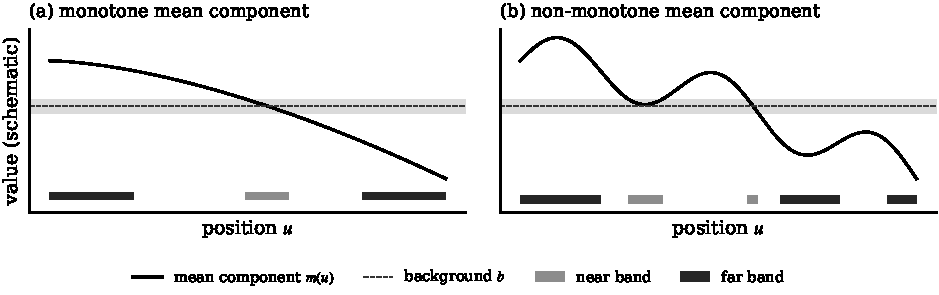
\includegraphics[width=\linewidth]{fig_state_bands.pdf}
\caption{Schematic of the bands of A1 and A2 for an unconditional background $b$. (a) Monotone mean component: the near band and the far band of the mean component map onto intervals of positions. (b) Non-monotone mean component: the same bands map onto scattered positions.}
\label{fig:bands}
\end{figure}

\paragraph{A3, spurious-pattern response.} A substitute at the background's value inside a window whose mean component is far from it creates an abrupt departure and return, which resembles a localized pattern of the process. A model that has learned to respond to such patterns responds to the one that masking created. In the monotone instance, a substitute toward the background in a late window resembles a temporary reversal of the mean component. In images, a convolutional network classified masked images by the pattern of the masks, predicting classes such as crossword puzzle \citep{jain2022missingness}, and masks optimized to delete evidence triggered artifacts of the network instead \citep{fong2017interpretable}; to our knowledge, no such response has been reported for time series. Under a target variable that depends only on the localized patterns, the target is zero on every window without a pattern, and since substitution inserts no patterns, the ground truth of such a window is zero under every background. \emph{M3} is the attribution mass $\sum|A_b(f)|$ on such windows. Its ideal value is 0.

\paragraph{A4, directional offset.} Masking pulls the model's reading of the window's mean component toward the background, so the signed change of the prediction depends on the sign of $b_c-m_{u,c}$. In the monotone instance, substituting late elements by values from the middle of the range moves predictions toward earlier states. In image classification, masking skewed the output distribution toward a few unrelated classes \citep{jain2022missingness}; to our knowledge, no directional effect of substitution has been reported for regression on mean-nonstationary data. \emph{M4} is the signed value-function distortion $\Delta_b(S)$ over the coalitions that the estimator evaluates, regressed on the state; its ideal slope and intercept are 0. Without a known function, M4 is the centring of $f(\mask(x_W,S,b))-f(x_W)$ within strata of the state index. If the substitute is unbiased for the masked value at the window's state, this shift is centred on zero to first order in $f$, so a systematic sign identifies a biased background.

\paragraph{A5, recurrent carry-over.} In a recurrent model, a substituted position alters the hidden state and therefore the processing of every later position, so the distortion is not confined to the masked element. To our knowledge, this propagation has not been reported for substitution-based attribution. For a position $u_0$ substituted on all channels, with $\tilde x^{(u_0)}_W$ the window after substitution, \emph{M5} is the change this causes in the distortion at the other positions,
\begin{equation}\label{eq:m5}
\mathrm{M5}(\ell) = \mathbb{E}\sum_c \bigl|D_b(\tilde x^{(u_0)}_W)_{u_0+\ell,c}-D_b(x_W)_{u_0+\ell,c}\bigr|, \qquad \ell\neq 0,
\end{equation}
compared between a recurrent model and a non-recurrent control. For an affine $g$ and a coalition-independent $b$, the ground truth at $u\neq u_0$ does not change, so carry-over appears as an excess of M5 at $\ell>0$ over $\ell<0$ in the recurrent model that the control does not show.

\paragraph{A6, coalition compounding.} Shapley values evaluate coalitions in which many elements are masked at once, so A1--A5 act together within one model call, and a coalition of many substitutes can leave the support even where each substitute alone would not. Off-manifold evaluation has been studied for the coalitions of Shapley values and for permuted features \citep{frye2021shapley, hooker2021unrestricted}; to our knowledge, how its effect grows with the number of substituted elements has not been reported. \emph{M6} compares $|\Delta_b(S)|$, as a function of the number of masked elements $|W\setminus S|$, with the sum of the single-element distortions $\sum_{i\in W\setminus S}|\Delta_b(W\setminus\{i\})|$. Growth above that sum is compounding.


%==============================================================================================
\section{Trend-aware backgrounds}
\label{sec:tab}
%==============================================================================================

Each background fixes what its attributions sum to (Equation~\eqref{eq:efficiency}), so the backgrounds below differ in the question they answer as well as in their distortion (Table~\ref{tab:explained}). Figure~\ref{fig:toy} shows the substitutes of four of them on one window, together with the sum of the exact attributions of an affine function under each.

\begin{table}[t]
\caption{What each background explains. Second column: the window on which $f$ is evaluated when all elements are masked; third: the sum of the attributions (Equation~\ref{eq:efficiency}).}
\label{tab:explained}
\centering
\small
\begin{tabularx}{\linewidth}{@{}>{\raggedright\arraybackslash}p{2.6cm}>{\raggedright\arraybackslash}p{3.2cm}>{\raggedright\arraybackslash}p{3.0cm}>{\raggedright\arraybackslash}X@{}}
\toprule
Background & All elements masked: $f$ evaluated on & Attributions sum to & Question answered \\
\midrule
B0, B1, B-pristine (unconditional) & a constant window $b$ & $f(x_W)-f(b)$ & Why does this prediction differ from a fixed reference? \\
B2, TAB-state (fine bins) & the population at this window's states & $f(x_W)-f(b_{\mathrm{state}}(x))$ & Why does it differ from a typical sequence at the same state? \\
B3, TAB-traj & the extrapolation of the sequence's own mean component & $f(x_W)-f(b_{\mathrm{traj}}(x))$ & What do the observations add beyond the sequence's own past? \\
B2c, B4 (coalition-dependent) & the population marginal & $f(x_W)-f(b_1)$, B4 approximately & The B1 question, with coalitions that stay on the data support \\
\bottomrule
\end{tabularx}
\end{table}

\begin{figure}[t]
\centering
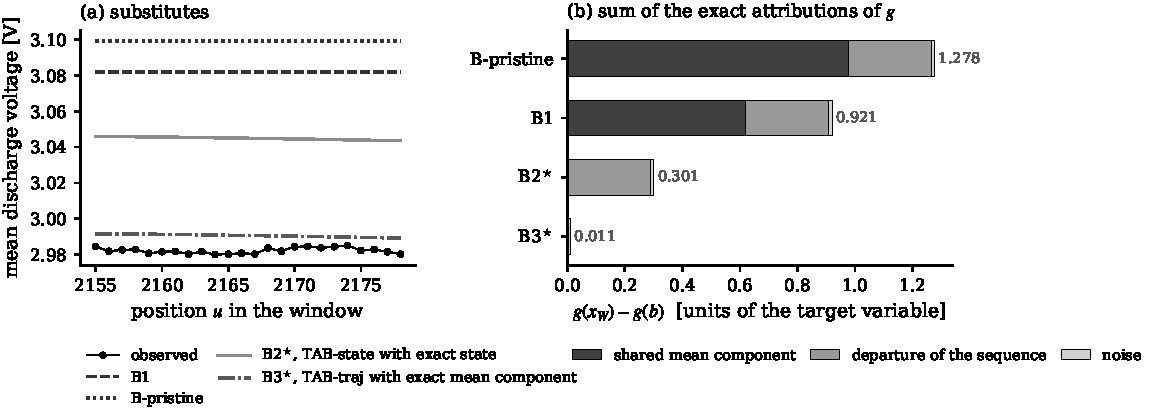
\includegraphics[width=\linewidth]{fig_toy_window.pdf}
\caption{One window ($L:=24$) of a sequence generated by DegradX's HUST profile, the evaluation window with the largest final degradation state among the profile's 120 \citep{degradx2026}. (a) Observed mean discharge voltage and the substitute of each background; B2$^\star$ and B3$^\star$ are TAB-state and TAB-traj with the exact state and the sequence's exact mean component. (b) Sum of the exact attributions of DegradX's affine reference model under each background, split into the parts due to the mean component shared by the sequences of the profile, the sequence's departure from it, and the noise.}
\label{fig:toy}
\end{figure}

\paragraph{B0, B1 and B-pristine.} Attributions are computed in raw input space: the model is wrapped with its input standardization, so that every background is specified in the units of the data. Zero after standardization is the training mean, that is, B1; \emph{B0} is therefore zero in raw units, a floor reference. \emph{B1} is the per-channel mean over all positions of the training sequences; TimeSHAP's average event, which its implementation computes as the per-channel median \citep{bento2021timeshap}, is reported as a variant.
% TODO: D3 default "the mean, as in the ACIIDS paper's Eq. 3" not verified (paper not available); the text states the mean without the ACIIDS reference.
By Equation~\eqref{eq:excess}, B1 has the smallest expected squared substitution distance of all backgrounds that are constant over positions and states, so comparing it with B0 and B-pristine varies the substitution distance while the stationarity assumption stays the same. \emph{B-pristine} places at every position the initial value $x^0_c$ of the mean component shared by the population, which DegradX calls the pristine reference point and uses as its primary baseline \citep{degradx2026}.

\paragraph{B2, TAB-state.} TAB-state substitutes the population mean of the channel among training observations at the same state. The state index of Equation~\eqref{eq:stateindex} is partitioned into $K$ bins $Q_1,\dots,Q_K$ by quantiles over the training sequences. With $k(u;x)$ the bin of $h_u(x)$,
\begin{equation}\label{eq:tabstate}
b^{\mathrm{state}}_c(u;x) = \frac{\sum_{j}\sum_{v}\mathbf{1}\{h_v(x_j)\in Q_{k(u;x)}\}\,x_{j,v,c}}{\sum_{j}\sum_{v}\mathbf{1}\{h_v(x_j)\in Q_{k(u;x)}\}},
\end{equation}
where $j$ runs over training sequences and $v$ over their positions. $b^{\mathrm{state}}$ is the binned estimate of the state-conditional mean $\mathbb{E}[x_{v,c}\mid h_v\in Q_k]$, which replaces the population mean that B1 estimates. The index is computed from $x_{1:u-1}$ rather than $x_{1:u}$: otherwise the masked value would feed its own substitute. Bins below a minimum count are merged with their neighbour along the index. When several channels are mean-nonstationary, the coordinates of $h$ are selected on the training split: each channel's causal running summary is scored by its association with elapsed position within sequences, near-duplicates of a higher-scoring summary are removed, and the best remaining summaries are kept up to the cap $d$. A robust variant replaces the bin mean by the bin median. The table of bin means is computed once, and each substitute is a lookup.

$K$ changes the question, not only the balance between bias and variance. With $K=1$, $b^{\mathrm{state}}$ equals B1 and keeps the mean component in what is explained. As $K$ grows, the substitute approaches the state-conditional mean $\mu_c$ at the window's state, and the attributions sum to what distinguishes the sequence from a typical sequence at that state: the part of its mean component specific to it, its localized patterns and its noise.

TAB-state assumes that (S1) conditioning on $h$ reduces the spread of $x_{u,c}$, diagnosed by the within-bin variance as a fraction of the total; (S2) sequences share one law of observation given the state, although they may differ in pace, diagnosed by the dispersion between sequences within a bin; (S3) every visited bin holds enough training observations, reported as the occupancy of the bins, with extreme states the most exposed; and (S4) $h$ is computable from $x_{1:u-1}$ without the target variable (R1). It assumes no shape of the mean component and needs no history of the sequence beyond the short window of $h$. It blurs across fast changes of the mean component, treats two sequences at the same state alike, and coarsens when the law of observation depends on the path beyond the state.

\paragraph{B3, TAB-traj.} TAB-traj substitutes the one-step extrapolation of the sequence's own mean component, fitted on its strict past. For channel $c$ and position $u$ with $u-1\ge t_{\min}$,
\begin{equation}\label{eq:tabtraj}
\hat m^{(u)}_c = \arg\min_{m\in\mathcal{M}} \sum_{v=1}^{u-1}\omega(u-v)\bigl(x_{v,c}-m(v)\bigr)^2 + \lambda P(m),
\qquad b^{\mathrm{traj}}_c(u;x) = \hat m^{(u)}_c(u),
\end{equation}
with a family $\mathcal{M}$ of smooth functions able to express sharp local curvature, a weight profile $\omega$, a roughness penalty $P$ and its weight $\lambda$, selected by cross-validation over training sequences. Below $t_{\min}$, TAB-traj falls back to TAB-state at the same position. The fit uses positions up to $u-1$ for two reasons. Including $x_{u,c}$ would make the substitute a smoothed copy of the value that masking is meant to remove, an under-perturbation that blunts the method by construction. Under the working decomposition $x_{v,c}=m(v)+\eta_v$ with $\mathbb{E}[\eta_v\mid x_{1:v-1}]=0$, the strict-past fit estimates $\mathbb{E}[x_{u,c}\mid x_{1:u-1}]$, so masking removes exactly the part of the observation that its own past does not predict. The fits are computed once per sequence, channel and position and reused across coalitions.

TAB-traj assumes that (T1) the decomposition above holds, diagnosed by the autocorrelation and the mean of the fit residuals; (T2) $\mathcal{M}$ can express the curvature present, diagnosed by the fit residuals stratified by position, since a spike in them marks a substitute that may itself lie off the support; (T3) the strict past is long enough and informative about $u$, with no unannounced change at $u$; and (T4) the noise is small relative to the movement of the mean component, otherwise the fit's variance enters the substitute. It needs no population of sequences. Its cost is a shift in meaning: an element that only confirms the predictable course of the sequence receives little attribution even if the model depends heavily on the mean component that the element carries. This answers a different question from that of an analyst who asks how much the mean component at that element matters.

Both TAB backgrounds therefore shift what is explained (Table~\ref{tab:explained}). With fine bins, TAB-state removes the population's mean component and explains the sequence's departures from it; TAB-traj removes the sequence's own mean component and explains what its past does not predict.

\paragraph{Oracles B2$^\star$ and B3$^\star$.} On generated data, where the state and the mean component are known exactly, two oracle backgrounds replace the estimates by the exact quantities. B2$^\star$ is the mean component shared by the sequences at the exact state, which TAB-state approaches with a perfect index and fine bins; B3$^\star$ is the sequence's exact mean component, which TAB-traj approaches with a perfect fit. They bound what TAB can reach, and the gap from B2 to B2$^\star$ is the estimation error of the state index. Since they drop the stationarity assumption without estimation error, they also test the thesis most directly. Their explained quantities are those of TAB-state with fine bins and of TAB-traj (Table~\ref{tab:explained}). Figure~\ref{fig:tabs} contrasts the two on one sequence.

\begin{figure}[t]
\centering
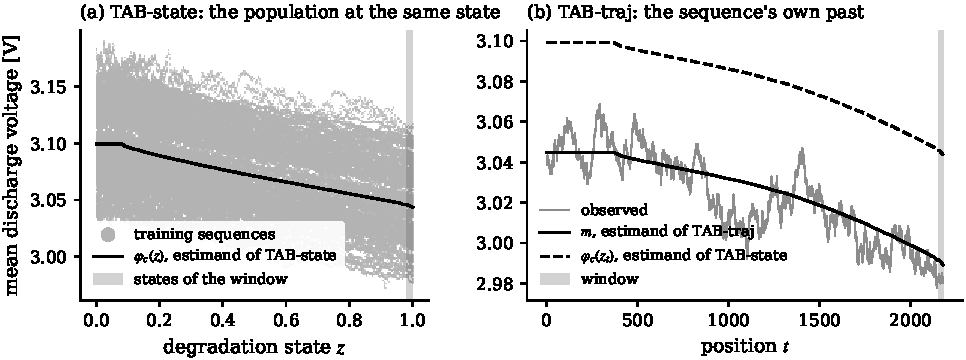
\includegraphics[width=\linewidth]{fig_tab_state_traj.pdf}
\caption{TAB-state against TAB-traj at their exact estimands, for the sequence and channel of Figure~\ref{fig:toy}. (a) The channel over all training sequences of the profile against their exact degradation state, with the mapping $\varphi_c(z)$ shared by the sequences \citep{degradx2026}, the estimand of TAB-state; the band marks the states of the window. (b) The channel of the sequence up to the end of the window, with its own mean component $m$, the estimand of TAB-traj, and $\varphi_c(z_t)$; the shaded positions are the window.}
\label{fig:tabs}
\end{figure}

\paragraph{B2c, coalition-conditional TAB.} B2c, a variant of TAB-state, keeps B1's explained quantity while keeping the coalitions near the window's own mean component. Each masked element takes the mean of the retained elements of the same channel in the window; a channel masked entirely takes the training mean $b_{1,c}$,
\begin{equation}\label{eq:b2c}
b^{\mathrm{2c}}_c(u;S) = \begin{cases}
\frac{1}{|S_c|}\sum_{(v,c)\in S_c} x_{v,c}, & S_c\neq\emptyset,\\
b_{1,c}, & S_c=\emptyset,
\end{cases}\qquad S_c = \{(v,c')\in S : c'=c\}.
\end{equation}
When all elements are masked, the window equals that of B1, so the attributions sum to $f(x_W)-f(b_1)$. B2c depends on the coalition and is therefore not covered by (R2); it assumes that the mean component changes little within a window, and where it does change, the substitute is the window's average rather than the mean component at the masked position.

\paragraph{B4, learned conditional imputer.} B4 is the generative on-manifold remedy of the Shapley literature \citep{frye2021shapley}, instantiated for windows. It is an established reference, not a contribution, and is not assumed to dominate. An imputer trained on unmasked training windows fills the masked elements with their conditional mean given the retained ones; with no element retained, the fill is the population mean, so B4 approximately keeps B1's explained quantity. B4 depends on the coalition and requires one imputer call per coalition. Since the imputer is a second model whose misfit enters the substitute, its error on held-out masked elements is reported with every B4 result.

\paragraph{Choosing a background.} The two TAB backgrounds condition at different resolutions, and their weaknesses are largely complementary. Table~\ref{tab:guide} states the resulting guide; each row is a hypothesis.

\begin{table}[t]
\caption{Selection guide. Each row is a hypothesis.}
\label{tab:guide}
\centering
\small
\begin{tabularx}{\linewidth}{@{}>{\raggedright\arraybackslash}p{5.4cm}>{\raggedright\arraybackslash}p{2.6cm}>{\raggedright\arraybackslash}X@{}}
\toprule
Property of the data or question & Favours & Reason \\
\midrule
Many training sequences; short explained histories & TAB-state & bins are populated; TAB-traj unavailable below $t_{\min}$ \\
A single sequence, or a population without history & TAB-traj & needs no population \\
High noise in a channel & TAB-state & population averaging removes fit variance (T4) \\
Long histories; mean components that differ between sequences & TAB-traj & pooling would blur differences between sequences \\
Localized patterns present and used by the model & TAB-traj & conditioning on the sequence removes the manufactured pattern (A3) \\
Sharp changes of the mean component & neither clearly & TAB-state blurs across the change; TAB-traj lags behind it \\
Same state, different course (path dependence) & TAB-traj & the state alone does not determine the observation \\
Does the absolute mean component here matter? & B1, B-pristine, B2c or B4 & only these keep the mean component in what is explained \\
\bottomrule
\end{tabularx}
\end{table}


%==============================================================================================
\section{Evaluation methodology}
\label{sec:eval}
%==============================================================================================

Figure~\ref{fig:design} shows how the parts of the evaluation connect: synthetic arms, on which the ground truth of every background is exact, and measured arms and a case study, which use the instruments that need no ground truth.

\begin{figure}[t]
\centering
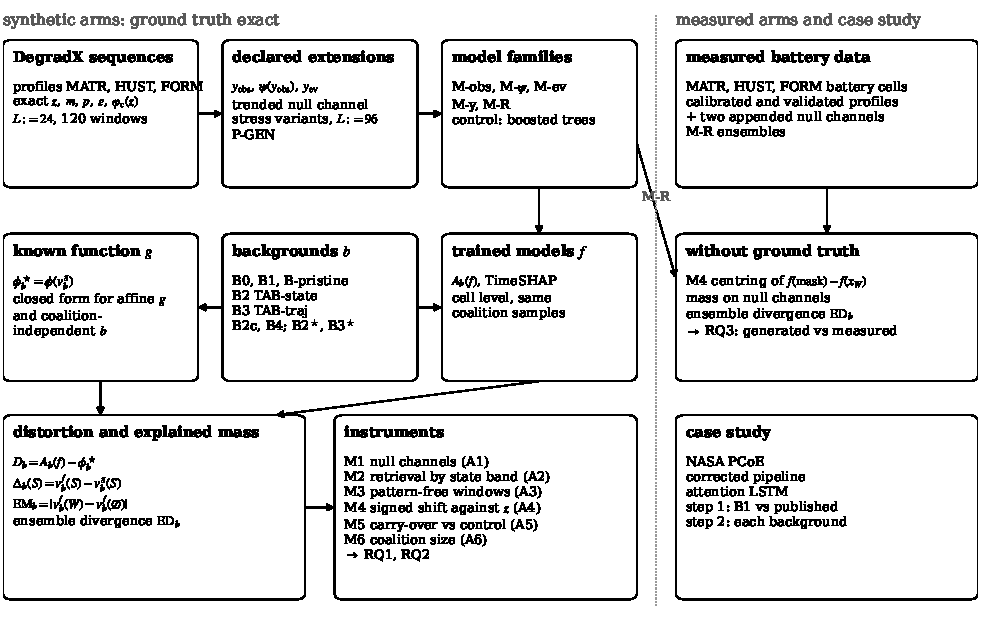
\includegraphics[width=\linewidth]{fig_eval_design.pdf}
\caption{Evaluation design. Generated sequences of the three DegradX profiles train the model families; each background yields a ground truth $\phi^\star_b$ on the known function and a distortion $D_b$ on the trained models, read through the instruments M1--M6 beside the explained mass. Measured battery data and the case study are read with the instruments that need no ground truth.}
\label{fig:design}
\end{figure}

\subsection{Ground truth per background}\label{sec:eval:gt}

\paragraph{Why each background needs its own ground truth.} A ground truth common to all backgrounds cannot decide between them. Each background fixes its own explained quantity (Equation~\eqref{eq:efficiency}), so a common ground truth would count a change of question as error. On trained models, moreover, such a ground truth does not even separate attribution methods. On DegradX, ten equally accurate LSTMs differ more than the attribution methods do in all but one case: in rank agreement, the methods differ by at most 0.073, whereas each method's range over the ten models is at least 0.099, and 0.32 to 0.34 in FORM. Switching TimeSHAP's background moved its rank agreement by at most 0.04, which was enough to change its place among the methods in two of the three profiles \citep{degradx2026}. A comparison of backgrounds scored in this way would be decided by which model happened to be trained.

\paragraph{A known function.} Each model is therefore trained on a target variable that is a known function $g$ of the observed window. On the support of its training data, a model that fits this target reproduces $g$, so the ground truth $\phi^\star_b$ of Equation~\eqref{eq:gt} is exact for every background, and $D_b$ separates the model's off-support response from the information that the background removes. For an affine $g(x_W) = \beta_0 + \sum_{(u,c)\in W} w_{u,c}\,x_{u,c}$ and a coalition-independent $b$, the game $v^g_b$ is additive, and $\phi^\star_{b,u,c} = w_{u,c}\,(x_{u,c}-b_c(u;x))$ in closed form. Otherwise, $\phi^\star_b$ is computed by permutation sampling of $g$, which is cheap to evaluate, so its sampling error can be made negligible against the distortion and is reported. The ground truth of every background is thus exact by construction, but no background is correct by construction: its distortion vanishes only if its substituted windows keep $f$ on its support, which a coalition of many smooth, noise-free substitutes need not do (A6). This removes the circularity for which DegradX declined backgrounds conditioned on the local mean component \citep{degradxrepo}. $D_b$ is reported in units of the target variable as $\|D_b\|_1=\sum_{(u,c)}|D_{b,u,c}|$ and relative to $\|\phi^\star_b\|_1$, always beside $\EM_b$.

\paragraph{Ensemble divergence.} Equally accurate models $f_1,\dots,f_n$ that all reproduce $g$ on the support can differ in their attributions under $b$, beyond their residual misfit, only through their responses to substituted windows off the support, just as off-manifold Shapley values differ between models that evaluate identically on the data \citep{frye2021shapley}. We introduce the \emph{ensemble divergence}
\begin{equation}\label{eq:ed}
\ED_b(x) = \sum_{(u,c)\in W} \operatorname{sd}_{k=1,\dots,n}\bigl(A_b(f_k)_{u,c}\bigr),
\end{equation}
the sum over elements of the across-model standard deviation, computed with the same coalition samples for every model. It measures how much an explanation depends on behaviour that the training data do not constrain, needs no ground truth, and therefore applies unchanged to models of measured data. It carries DegradX's ensemble range, the range of a score over ten equally accurate models \citep{degradx2026}, from scores to attribution maps.

\paragraph{How the thesis is tested.} If the stationarity assumption of an unconditional background is what distorts the attribution, three consequences follow, and each is read from the instruments. (i) Under the unconditional backgrounds, the distortion is structured by the systematic substitution distance: on elements of zero ground truth it grows with $d_{u,c}$ (M1), the retrieval of localized patterns differs between the near and the far band (M2), and the signed distortion follows the sign of $b_c-m_{u,c}$ along the state (M4). B0, B1 and B-pristine share the assumption but lie at different distances from the mean component at every state, so this structure must follow the distance rather than the background. (ii) Backgrounds that drop the assumption reduce the distortion: TAB-state and TAB-traj, and most directly the oracles B2$^\star$ and B3$^\star$, which drop it without estimation error. Each reduction is read beside the explained mass, so that a background is not credited for explaining less. (iii) The structure follows the mean component rather than position, so it persists on generated data whose mean component is not monotone in position. The thesis is contradicted if the distortion under unconditional backgrounds is unrelated to the substitution distance, or if the oracles do not reduce it; the distortion would then have a source other than the stationarity assumption. A reduction under the oracles but not under TAB would place the failure in the estimation of the state rather than in the thesis. RQ1 tests consequences (i) and (iii), and RQ2 tests consequence (ii) together with the comparison with B4. Every instrument is therefore computed under every background: RQ1 reads its value under the unconditional backgrounds, and RQ2 its paired difference under the others.

\subsection{Testbed and its extensions}\label{sec:eval:testbed}

\paragraph{DegradX as used.} DegradX \citep{degradx2026} generates multivariate sequences, which it calls units, from profiles fitted to the battery datasets MATR \citep{severson2019data}, HUST \citep{ma2022real} and FORM \citep{cui2024data}. Each channel of a generated sequence is $x_{t,c} = m_{t,c}+\sum_k p_{k,t,c}+\varepsilon_{t,c}$, the sum of a mean component, inserted patterns and noise, with $m_{t,c}=\varphi_c(z_t)+\delta_{c,i}$. Here $z_t$ is the degradation state, DegradX's state, which runs from 0 at an early-life reference to 1 at end of life; $\varphi_c$ is a monotone mapping shared by the sequences of a profile, and $\delta_{c,i}$ is a per-sequence offset \citep{degradx2026}. The profiles, their generator and seeds, and the exact decomposition of every sequence are used unchanged: $z$, $m$, $p$, $\varepsilon$, and $\varphi_c(z)$ without offsets, which the repository records for every sequence \citep{degradxrepo}. So are the reference model
\begin{equation}\label{eq:refmodel}
g(x_W) = \sum_{(u,c)\in W} w_{u,c}\,\bigl(x_{u,c}-x^0_c\bigr), \qquad x^0_c = \varphi_c(0),
\end{equation}
with weights $w_{u,c}=\kappa_c\pi_u$, the product of a channel factor and DegradX's recency profile $\pi_u\propto 2^{-(t-u)/h}$, with $L:=24$ and the half-life $h:=L/4=6$; the two null channels, which do not depend on the degradation state, and DegradX's checks that a model does not use them; the ten-member LSTM ensembles of hidden size 64 with two layers and hidden size 128 with one layer, five initializations each \citep{degradxrepo}; the scores; the TSTR ratio of each profile; and the 120 evaluation windows of each profile \citep{degradx2026}. Models use the 300 sequences of generation seed 0, 210 for training, 45 for validation and 45 for testing \citep{degradx2026}. On DegradX, B-pristine is $x^0_c$ at every position, and the oracles are B2$^\star_c(u) = \varphi_c(z_u)$ and B3$^\star_c(u) = m_{u,c}$.

\paragraph{The premise in the testbed.} Figure~\ref{fig:distance} shows the two terms of Equation~\eqref{eq:excess} on the testbed: for every profile and weighted channel, the systematic substitution distance of B1 and B-pristine from the population's state-conditional mean, relative to the spread of the observations at each degradation state. B1 lies close to the population only around one state, and B-pristine only near the start; away from these states, the distance grows. On capacity, whose spread at a given state is small, the distance far exceeds that spread over most states; on the other weighted channels, whose spread includes the offsets of the sequences, it is smaller and follows the same course. The figure describes the input data only, not any attribution. The models, in turn, read the state: every weighted channel is used by all ten models of every profile, and DegradX's target depends on the mean component apart from a pattern term that is absent in MATR and HUST and negligible in FORM \citep{degradx2026}.

\begin{figure}[t]
\centering
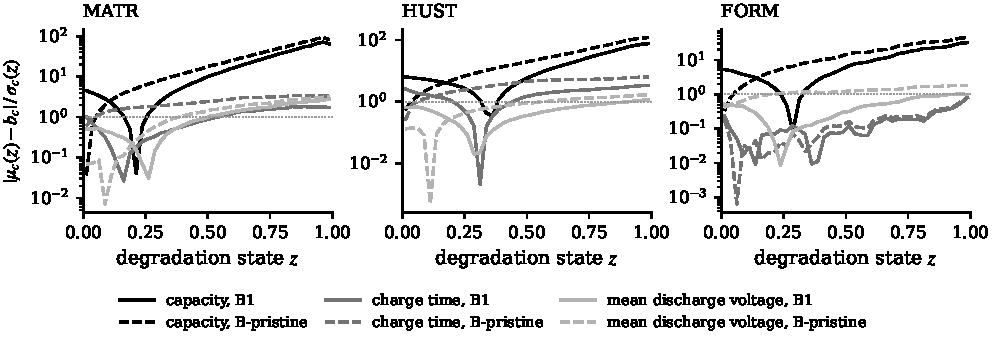
\includegraphics[width=\linewidth]{fig_substitution_distance.pdf}
\caption{Distance of the unconditional backgrounds B1 (solid) and B-pristine (dashed) from the population at each degradation state $z$, for the weighted channels of each DegradX profile: $|\mu_c(z)-b_c|/\sigma_c(z)$, with $\mu_c(z)$ and $\sigma_c(z)$ the mean and standard deviation of the channel over the training sequences of generation seed 0 in 40 equal-width bins of $z$. The dotted line marks one standard deviation.}
\label{fig:distance}
\end{figure}

\paragraph{Declared extensions.} DegradX is not modified; the following extensions are added on top of it, each labelled where its results appear.
\begin{itemize}
\item \emph{Two target variables.} The observation-level target $y_{\mathrm{obs}} = g(x_W)$, the reference model applied to the observed window, noise included; and, conditional on the pilot, $\psi(y_{\mathrm{obs}})$ for a monotone nonlinear $\psi$.
\item \emph{A trended null channel.} M1 needs channels that are mean-nonstationary but have zero ground truth, here called trap channels. A zero-weight channel that carries the degradation state cannot serve as one. In MATR, whose zero-weight channels internal resistance and temperature carry the state, the share of attribution on zero-weight channels is 0.134 to 0.198, against at most 0.048 in HUST and FORM, whose zero-weight channels are the null channels \citep{degradx2026}. A channel that carries the state predicts the target variable, so a model can reproduce $g$ on the support while reading it, and its attribution then reflects which function the model learned rather than a substitution artifact. The trended null channel is therefore independent of the sequence's state: the degradation-state trajectory of another generated sequence, read from a random starting position, held at its end-of-life value after that sequence ends, mapped through the profile's charge-time mapping and given noise of the charge-time variance and autocorrelation. It has zero target weight, and it is accepted only if it passes DegradX's null-channel check and its conditional channel-use check on every model.
\item \emph{An event-driven target on FORM.} A3 needs a model that responds to localized patterns. FORM's inserted patterns carry $1.7\times10^{-5}$ of the variance of the mean term, and removing them from DegradX's target leaves the error of trained models unchanged \citep{degradx2026}, so a model trained on $y$ has no reason to respond to them. The event-driven target $y_{\mathrm{ev}} = \sum_{(u,c)\in W} w_{u,c}\sum_k p_{k,u,c}$ is the sparse part of DegradX's target alone. Its ground truth on windows without patterns is zero everywhere.
\item \emph{Stress variants}, made with DegradX's existing generator overrides at the values of its declared grids: transition sharpness $z\mapsto z^s$, $s\in\{0.25,0.5,1,2,4\}$; noise-variance multiplier $\in\{0.25,0.5,1,2,4,8,16\}$; and pattern-amplitude multiplier $\in\{0.25,0.5,1,2,4,8\}$ \citep{degradxrepo}. They are not calibrated to any dataset.
\item \emph{One longer window}, $L:=96$ from DegradX's declared grid of window lengths \citep{degradxrepo}, for A5 and for profiles of attribution within a window.
% TODO: D2 -- use the sequence length of the ACIIDS paper if that paper states one (paper not available); 96 is the stated default.
\item \emph{A non-monotone probe}, P-GEN: a slow periodic component added to the mean component of the weighted channels, so that the mean component is not monotone in position. DegradX's generator is monotone by construction, so P-GEN requires new generator code. Under $y_{\mathrm{obs}}$ the periodic component enters the target variable. P-GEN tests consequence (iii) of the thesis and is not calibrated.
\end{itemize}

\subsection{Models}\label{sec:eval:models}

\paragraph{Model families.} All models are DegradX's LSTM regressor, trained with DegradX's procedure in ten-member ensembles of the two architectures above \citep{degradxrepo}, except the control.
\begin{itemize}
\item \emph{M-obs}, trained on $y_{\mathrm{obs}}$, the primary family. Because $y_{\mathrm{obs}}$ is a deterministic function of the input window, a model that fits it reproduces $g$ on the support. A function-identity check confirms this for every member: on the windows of held-out generated sequences, the root-mean-square difference between $f$ and $g$ must lie within a fraction $\vartheta$ of the standard deviation of $\sum w\varepsilon$, the part of $y_{\mathrm{obs}}$ that a model of $y$ could not predict. Accuracy alone does not establish this: DegradX's ten equally accurate models need not learn the function that defines its ground truth, since the channels of a window share one degradation state and other functions reproduce the target equally well \citep{degradx2026}.
\item \emph{M-$\psi$}, trained on $\psi(y_{\mathrm{obs}})$, conditional on the pilot. It covers the possibility that an LSTM fitted to an affine function stays nearly linear off its support, which would make every distortion small. Its ground truth is the Shapley value map of $\psi\circ g$, computed by permutation sampling.
\item \emph{M-ev}, trained on $y_{\mathrm{ev}}$ on FORM, for M3.
\item \emph{M-y}, DegradX's released ensembles trained on $y$, read only with instruments that need no ground truth.
\item \emph{M-R}, trained on the RUL target $R$ of DegradX \citep{degradx2026}. Its inputs are the channels plus elapsed position, which is unmasked context rather than a player, since masking elapsed position with a population mean would be an A1 case of its own and would dominate. M-R ensembles are trained both on generated sequences and on measured battery cells.
\item \emph{The control}, gradient-boosted regression trees \citep{friedman2001greedy} on flattened windows, trained on $y_{\mathrm{obs}}$ at the longer $L$ together with an M-obs ensemble at that $L$; having no recurrent state, it is the non-recurrent control of M5.
\end{itemize}
For M-obs and every coalition-independent background, the ground truth is $\phi^\star_{b,u,c} = w_{u,c}(x_{u,c}-b_c(u;x))$; for B2c, B4 and M-$\psi$ it is computed by permutation sampling of the known function. The verdict on RQ1 and RQ2 rests on $D_b$ on M-obs, reported with $\EM_b$, as paired contrasts within models together with the number of members that agree in sign.

\subsection{Instruments, predictions and statistics}\label{sec:eval:instruments}

\paragraph{Instruments on DegradX.} Table~\ref{tab:instruments} gives the realization of each instrument. Ensemble divergence, explained mass and DegradX's scores against $\phi^\star_b$, namely rank agreement, channel allocation error and temporal profile error \citep{degradx2026}, are computed on every arm where they are defined.

\begin{table}[t]
\caption{Realization of the instruments on DegradX. $z$: exact degradation state.}
\label{tab:instruments}
\centering
\small
\begin{tabularx}{\linewidth}{@{}l>{\raggedright\arraybackslash}X>{\raggedright\arraybackslash}p{2.7cm}@{}}
\toprule
Artifact & Instrument & Models \\
\midrule
A1 & M1 on the two null channels and the trended null channel & M-obs, M-$\psi$; M-y, M-R on null channels \\
A2 & M2 on FORM, whose inserted patterns enter $y_{\mathrm{obs}}$ linearly; bands set by $z$ & M-obs (FORM) \\
A3 & M3 on windows without patterns, ground truth 0 & M-ev (FORM) \\
A4 & M4 against $z$: $f(\mask(x_W,S,b))-g(\mask(x_W,S,b))$; without $g$, centring of $f(\mask(x_W,S,b))-f(x_W)$ & all; centring only for M-y, M-R \\
A5 & M5 at $L:=96$, LSTM against the control & M-obs, control \\
A6 & M6 over the coalitions evaluated by the estimator & M-obs, M-$\psi$ \\
\bottomrule
\end{tabularx}
\end{table}

\paragraph{Predictions for the selection guide.} Each row of Table~\ref{tab:guide} is bound to an existing arm. (E1) TAB-traj's advantage over TAB-state grows with the available history and vanishes below $t_{\min}$, where the two coincide; read from $D_b$ stratified by $u-1$. (E2) TAB-state's advantage over B1 grows with the number of training sequences per bin; read from HUST against FORM on the measured arms, whose fitting splits hold 54 and 127 battery cells \citep{degradx2026}, and from nested random subsets of the generated training sequences, for which only the table of Equation~\eqref{eq:tabstate} is recomputed. (E3) Both TAB backgrounds degrade under sharp transitions, TAB-state by blur and TAB-traj by lag, distinguished by the fit residuals of (T2); read on the transition-sharpness variants. (E4) TAB-traj degrades faster than TAB-state as the noise variance grows; read on the noise-variance variants. (E5) TAB-state's correction shrinks more than TAB-traj's when the state no longer identifies the position; read on P-GEN. A falsified prediction corrects the guide.

\paragraph{Statistics.} Backgrounds are compared as paired contrasts within a model: on the same windows and with the same coalition samples of the estimator. Scores are averaged over the windows of a sequence and then over sequences, and intervals are 95\% bootstrap intervals over sequences, as in DegradX, with 10{,}000 bias-corrected and accelerated resamples \citep{degradx2026, degradxrepo}. Each contrast is reported with the number of the ten members whose contrast has the same sign. Instruments are stratified by the exact degradation state on generated sequences and by the state index on measured data.

\subsection{Measured data and case study}\label{sec:eval:measured}

\paragraph{Measured arms.} The measured arms use the battery cells of MATR \citep{severson2019data}, HUST \citep{ma2022real} and FORM \citep{cui2024data}, each with its calibrated and validated DegradX profile. The TSTR ratio of each profile states how far its synthetic arm stands for the dataset: 1.17 [0.94, 1.34] for HUST, whose interval contains one, and 1.49 [1.04, 2.29] and 1.54 [1.28, 1.74] for MATR and FORM, which reproduce part, but not all, of the dependence between the sequences and the RUL \citep{degradx2026}. M-R ensembles trained on the battery cells of the fitting splits are read with the instruments that need no ground truth: the centring of M4, the attribution mass on null channels, and ensemble divergence. Two null channels, constructed as DegradX constructs them for generated sequences, a constant plus noise with the autocorrelation of the capacity noise and the measured values of a channel permuted across battery cells and positions \citep{degradx2026}, are appended to the measured data, so that the measured arms also have channels of known irrelevance. B-pristine takes $x^0$ from the profile of the dataset. The same instruments are computed on M-obs, so that RQ3 can compare the signatures found there with those of M-R models trained on generated sequences and on measured battery cells of the same dataset. On measured data they can falsify a background, since a background that fails a necessary condition is biased, but cannot certify one; certification rests on the synthetic arms.

\paragraph{Case study.} The case study re-examines the authors' own published attribution findings on their own corrected pipeline \citep{mishchuk2026explaining}; it is not an audit of the literature, and no external reproduction is attempted. It uses the battery data set of the NASA Prognostics Center of Excellence (PCoE) \citep{saha2007battery} and the attention LSTM of the earlier study, which appears only here.
% TODO: PCoE battery cells and preprocessing, and the attention-LSTM architecture, from the ACIIDS paper (paper not available).
The pipeline is corrected so that normalization statistics are computed on training battery cells alone and no input depends on positions after the predicted one, the rules DegradX applies \citep{degradx2026}.
% TODO: state what the published pipeline did differently, from the ACIIDS paper (paper not available).
The study has two steps. Step~1 runs the corrected pipeline with the original background, B1, and compares the result with the published values, which isolates the effect of the correction. Step~2 runs the corrected pipeline with each background, which isolates the effect of the background. For each published finding, a table states whether it survives step~1, step~2, both or neither.
% TODO: list of the published findings, from the ACIIDS paper (paper not available).

\subsection{Implementation}\label{sec:eval:impl}

All attributions use TimeSHAP 1.0.4 at DegradX's declared settings: cell level, that is, one attribution per element, $\textit{nsamples}:=32{,}000$ and pruning off \citep{bento2021timeshap, degradxrepo}. Coalition-independent backgrounds are passed to TimeSHAP as a background sequence of the window's length, $L\times C$, which the TimeSHAP 1.0.4 kernel accepts as an alternative to a single background event; DegradX's wrapper tiles a single event over the window, and passing the sequence is its only change. B2c and B4 do not fit a single background, since their substitute depends on the coalition; they require a modified masking step in the kernel, which computes the substitute for each sampled coalition before the model is called. All backgrounds of a contrast share the coalition-sampling seed.

The background enters every substitution-based Shapley estimator only through $v_b$, since each such estimator computes attributions as weighted aggregations of differences of $v_b$. A1--A4 are properties of single model calls on substituted inputs, so their existence, sign and structure are common to the family, whereas their magnitudes depend on how an estimator weights coalition sizes, which interacts with A6; A5 is a property of the architecture. One synthetic arm, one profile under B0, B1 and B2, is therefore replicated with TSHAP, which computes SHAP values exactly for groups of time steps \citep{nguyen2025tshap}, and compared at the level of signatures: the sign of M1, the profile of M4 against the state, and the ranking of the backgrounds.
% TODO: TSHAP's applicability to the LSTM regressor and to element-level players not verified (v5.1 Sec. 9; no open copy of the paper).


%==============================================================================================
\section{Examples of citations, figures, tables, references}
\label{sec:others}
\lipsum[8] \cite{kour2014real,kour2014fast} and see \cite{hadash2018estimate}.

The documentation for \verb+natbib+ may be found at
\begin{center}
  \url{http://mirrors.ctan.org/macros/latex/contrib/natbib/natnotes.pdf}
\end{center}
Of note is the command \verb+\citet+, which produces citations
appropriate for use in inline text.  For example,
\begin{verbatim}
   \citet{hasselmo} investigated\dots
\end{verbatim}
produces
\begin{quote}
  Hasselmo, et al.\ (1995) investigated\dots
\end{quote}

\begin{center}
  \url{https://www.ctan.org/pkg/booktabs}
\end{center}


\subsection{Figures}
\lipsum[10] 
See Figure \ref{fig:fig1}. Here is how you add footnotes. \footnote{Sample of the first footnote.}
\lipsum[11] 

\begin{figure}
  \centering
  \fbox{\rule[-.5cm]{4cm}{4cm} \rule[-.5cm]{4cm}{0cm}}
  \caption{Sample figure caption.}
  \label{fig:fig1}
\end{figure}

\subsection{Tables}
\lipsum[12]
See awesome Table~\ref{tab:table}.

\begin{table}
 \caption{Sample table title}
  \centering
  \begin{tabular}{lll}
    \toprule
    \multicolumn{2}{c}{Part}                   \\
    \cmidrule(r){1-2}
    Name     & Description     & Size ($\mu$m) \\
    \midrule
    Dendrite & Input terminal  & $\sim$100     \\
    Axon     & Output terminal & $\sim$10      \\
    Soma     & Cell body       & up to $10^6$  \\
    \bottomrule
  \end{tabular}
  \label{tab:table}
\end{table}

\subsection{Lists}
\begin{itemize}
\item Lorem ipsum dolor sit amet
\item consectetur adipiscing elit. 
\item Aliquam dignissim blandit est, in dictum tortor gravida eget. In ac rutrum magna.
\end{itemize}


\section{Conclusion}
Your conclusion here

\section*{Acknowledgments}
This was was supported in part by......

%Bibliography
\bibliographystyle{unsrtnat}  
\bibliography{references}  


\end{document}
